\section{Lecture 6: Discovering acceleration}

In this lecture, we seek to find methods that converge faster than those
discussed in previous lectures. To derive this accelerated method, we start by
considering the special case of optimizing quadratic functions. Our exposition
loosely follows Chapter~$17$ in Lax's excellent text~\cite{lax}.

\subsection{Quadratics}

\begin{definition}[Quadratic function] A quadratic function $f\colon\R^n \to \R$ takes the form: 
\begin{equation*}
f(x) = \frac{1}{2}x^T A x - b^T x + c,
\end{equation*}
where $A \in S^n$, $b \in \R^n$ and $c \in \R$.
\end{definition}

%\begin{remark}
Note that substituting $n=1$ into the above definition recovers the familiar univariate quadratic function $f(x) = ax^2 + bx + c$ where $a, b, c \in \R$, as expected. There is one subtlety in this definition: we restrict $A$ to be symmetric. In fact, we could allow $A \in \R^{n \times n}$ and this would define the same class of functions, since for any $A \in \R^{n \times n}$ there is a symmetric matrix $\tilde{A} = \frac{1}{2}\left(A + A^T\right)$ for which:
\begin{equation*}
x^TAx = x^T \tilde{A} x\ \forall x \in \R^n.
\end{equation*}
Restricting $A \in S^n$ ensures each quadratic function has a \textit{unique} representation.

The gradient and Hessian of a general quadratic function take the form:
\begin{align*}
\nabla f(x) &= Ax - b \\
\nabla^2 f(x) &= A.
\end{align*}
Note provided $A$ is non-singular, the quadratic has a unique critical point at:
\begin{equation*}
x^* = A^{-1}b.
\end{equation*}
When $A \succ 0$, the quadratic is \textit{strictly convex} and this point is the unique global minima.

\subsection{Gradient descent on a quadratic}
In this section we will consider a quadratic $f(x)$ where $A$ is positive definite, and in particular that:
\begin{equation*}
\alpha I \preceq A \preceq \beta I,
\end{equation*}
for some $0 < \alpha < \beta$. This implies that $f$ is $\alpha$-strongly convex and $\beta$-smooth. 

From \theoremref{constrained_convergence_smooth_and_strongconvexity} we know that under these conditions, gradient descent with the appropriate step size converges linearly at the rate $\exp\left(-t \frac{\alpha}{\beta}\right)$. Clearly the size of $\frac{\alpha}{\beta}$ can dramatically affect the convergence guarantee. In fact, in the case of a quadratic, this is related to the \textit{condition number} of the matrix $A$.

\begin{definition}[Condition number]
Let $A$ be a real matrix. Its \textit{condition number} (with respect to the Euclidean norm) is:
\begin{equation*}
\kappa(A) = \frac{\sigma_{\max}(A)}{\sigma_{\min}(A)},
\end{equation*}
the ratio of its largest and smallest eigenvalues.
\end{definition}

So in particular, we have that $\kappa(A) \leq \frac{\beta}{\alpha}$; henceforth, we will assume that $\alpha, \beta$ correspond to the minimal and maximal eigenvalues of $A$ so that $\kappa(A) = \frac{\beta}{\alpha}$. It follows that gradient descent with a constant step size $\frac{1}{\beta}$ converges at:
\begin{equation*}
\left||x_{t+1} - x^*\right\|^2 \leq \exp{\left(-t \frac{1}{\kappa}\right)}\|x_1 - x^*\|^2.
\end{equation*}
In many cases, $f$ is ill-conditioned and $\kappa$ can easily take values in the hundreds or thousands. In this case, case convergence could be very slow: note that at $t > \kappa$, the error may have been reduced by only a factor of $3\times$. Can we do better than this?

In the case of a quadratic, we can of course use the analytic solution $x^* = A^{-1}b$. However, it will prove instructive to consider applying gradient descent to quadratic functions, and derive the convergence bound that we previously proved for any strongly convex smooth functions. This exercise will show us where we are losing performance, and suggest a method that can attain better guarantees.

\subsubsection{Convergence analysis}

\begin{theorem}
Assume $f\colon\R^n\to\R$ is a quadratic where the quadratic coefficient matrix has a condition number $\kappa$. Let $x^{*}$ be an optimizer of $f$, and let $x_{t}$ be the updated point at step $t$ using gradient descent with a constant step size $\frac{1}{\beta}$, i.e. using the update rule $x_{t+1} = x_t - \frac{1}{\beta}\nabla f(x_t)$. Then:
\begin{equation*}
\|x_{t+1} - x^*\|^2 \leq \exp\left(-t \frac{1}{\kappa}\right)\|x_1 - x^*\|^2.
\end{equation*}
\end{theorem}
\begin{proof}
Write:
\[
f(x) = \frac{1}{2}x^T A x - b^T x + c,
\]
where $A \in S^n$, $b \in \R^n$ and $c \in \R$. A gradient descent update with step size $\eta_t$ takes the form:
\[
x_{t+1} = x_t - \eta_t \nabla f(x_t) = x_t - \eta_t \left(Ax_t - b\right)
\]
Subtracting $x^*$ from both sides of this equation and using the property that $Ax^* - b = \nabla f(x^*) = 0$:
\begin{align*}
x_{t+1} - x^* &= \left(x_t - \eta_t\left(Ax_t - b\right)\right) - \left(x^* - \eta_t\left(Ax^* - b\right)\right) \\
&= (I - \eta_t A)(x_t - x^*)\\
&= \prod_{k=1}^t (I-\eta_k A)(x_1-x^*)\,.
\end{align*}
Thus,
\begin{align*}
\left\|x_{t+1} - x^*\right\|_2 &\leq \left\|\prod_{k=1}^t(I - \eta_t
A)\right\|_2 \left\|x_1 - x^*\right\|_2
\leq \left(\prod_{k=1}^t \left\| I - \eta_k A\right\|_2\right) \left\|x_1 - x^*\right\|_2.
\end{align*}

Set $\eta_k = \frac{1}{\beta}$ for all $k$. Note that $\frac{\alpha}{\beta}I \preceq \frac{1}{\beta}A \preceq I$, so:
\begin{equation*}
\max_{A \in \R^{n\times n}} \left\|I - \frac{1}{\beta} A\right \|_2 = 1 - \frac{\alpha}{\beta} = 1 - \frac{1}{\kappa}.
\end{equation*}
It follows that
\begin{align*}
\left\|x_{t+1} - x^*\right\|_2 &\leq \left(1 - \frac{1}{\kappa}\right)^t \left\|x_1 - x^*\right\|_2 
\leq \exp \left(-\frac{t}{\kappa}\right) \left\|x_1 - x^*\right\|_2.
\end{align*}
\end{proof}

\subsection{Accelerated gradient descent}
In the previous section, we proved an upper bound on the convergence rate. In this section, we would like to improve on this. Consider whether there was any point where we were careless in the proof above? One obvious candidate is that our choice of step size, $\eta_k = \frac{1}{\beta}$, was chosen rather arbitrarily. In fact, by choosing the sequence $\eta_k$ we can select \textit{any} degree-$t$ polynomial of the form:
\[
p(A) = \prod_{k=1}^t \left(I - \eta_k A\right).
\]

Note that:
\begin{equation*}
\left\|p(A)\right\| = \max_{x \in \lambda(A)} \left|p(x)\right|
\end{equation*}
where $p(A)$ is a matrix polynomial, and $p(t)$ is the corresponding scalar
polynomial. In general, we may not know the set of eigenvalues $\lambda(A)$, but
we do know that all eigenvalues are in the range $[\alpha, \beta].$ Relaxing
the upper bound, we get
\begin{equation*}
\left\|p(A)\right\| \le \max_{x \in [\alpha, \beta]} \left|p(x)\right|\,.
\end{equation*}
We can see now that we
want a polynomial $p(a)$ that takes on small values in $[\alpha, \beta],$ while 
satisfying the additional normalization constraint~$p(0) = 1.$ 

\subsubsection{A naive polynomial solution}
A naive solution chooses a uniform step size $\eta_t = \frac{2}{\alpha + \beta}$. Note that
\[
\max_{x \in [\alpha, \beta]} \left|1 - \frac{2}{\alpha + \beta} x\right| = \frac{\beta - \alpha}{\alpha + \beta} \leq \frac{\beta}{\alpha} = \kappa,
\]
recovering the same convergence rate we proved previously.
\begin{figure}[h]
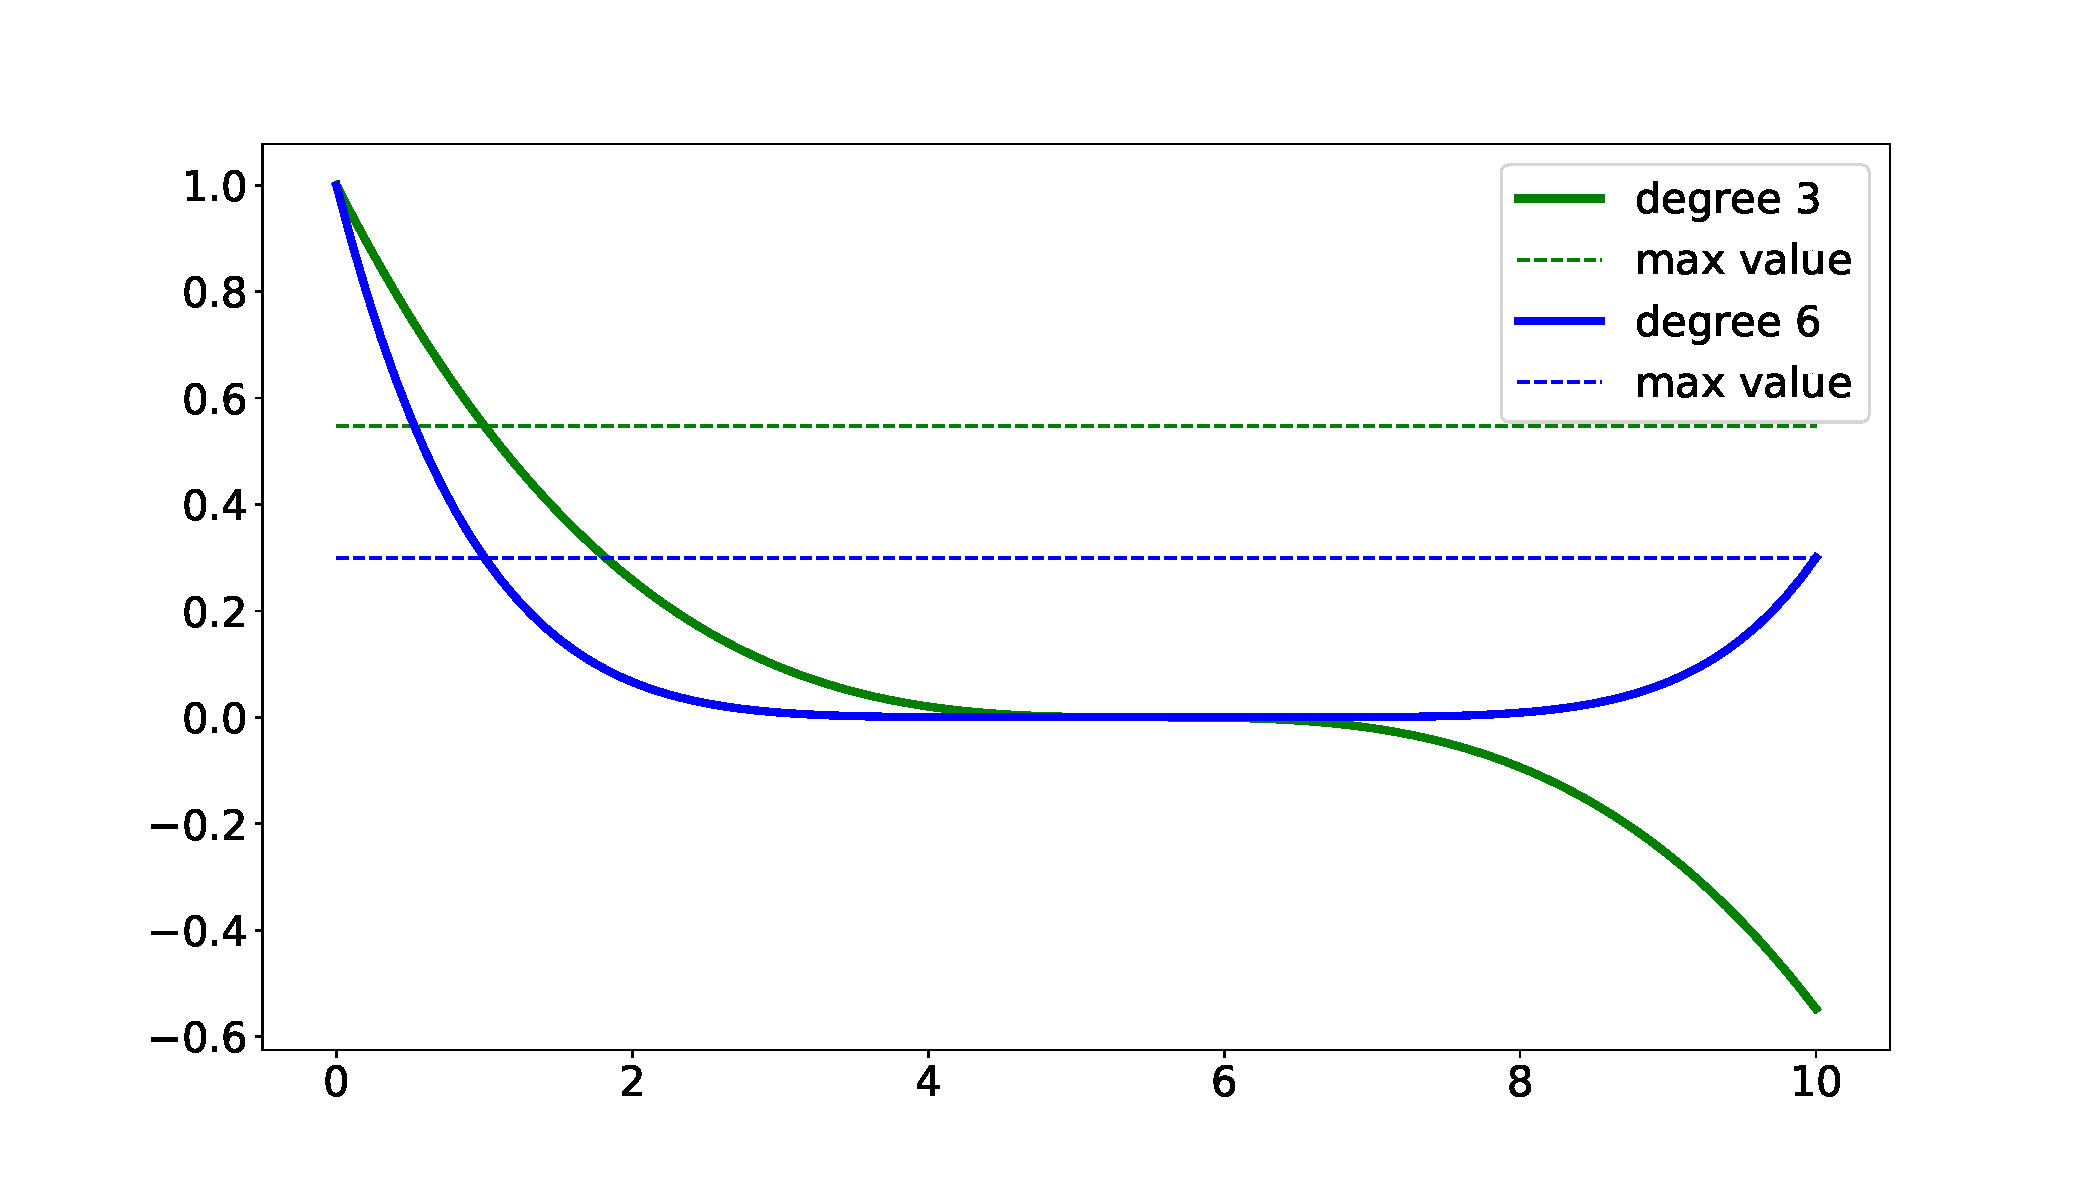
\includegraphics[width=0.9\textwidth]{figures/lecture6-naive_polynome.pdf}
\centering
\caption{Naive Polynomial}
\label{naive_p}
\end{figure}
%
The resulting polynomial $p_t(x)$ is plotted in Figure~\ref{naive_p} for degrees
$t = 3$ and $t = 6$, with $\alpha = 1$ and $\beta = 10$. Note that doubling the
degree from three to six only halves the maximum absolute value the polynomial
attains in $[\alpha,\beta]$, explaining why convergence is so slow.

\subsection{Chebyshev polynomials}
%
Fortunately, we can do better than this by speeding up gradient descent using
Chebyshev polynomials. The Chebyshev polynomials are a sequence of orthogonal
polynomials which are related to de Moivre's formula and which can be defined
recursively. We will use Chebyshev polynomials of the first kind,
defined by the recurrence relation:
\begin{align*}
T_0(a) &= 1,\quad T_1(a) = a \\
T_k(a) &= 2a T_{k-1}(a) - T_{k-2}(a),\ \text{for }k \geq 2\,.
\end{align*}
Figure \ref{chebychev_poly} plots the first few Chebyshev polynomials.

\begin{figure}[ht]
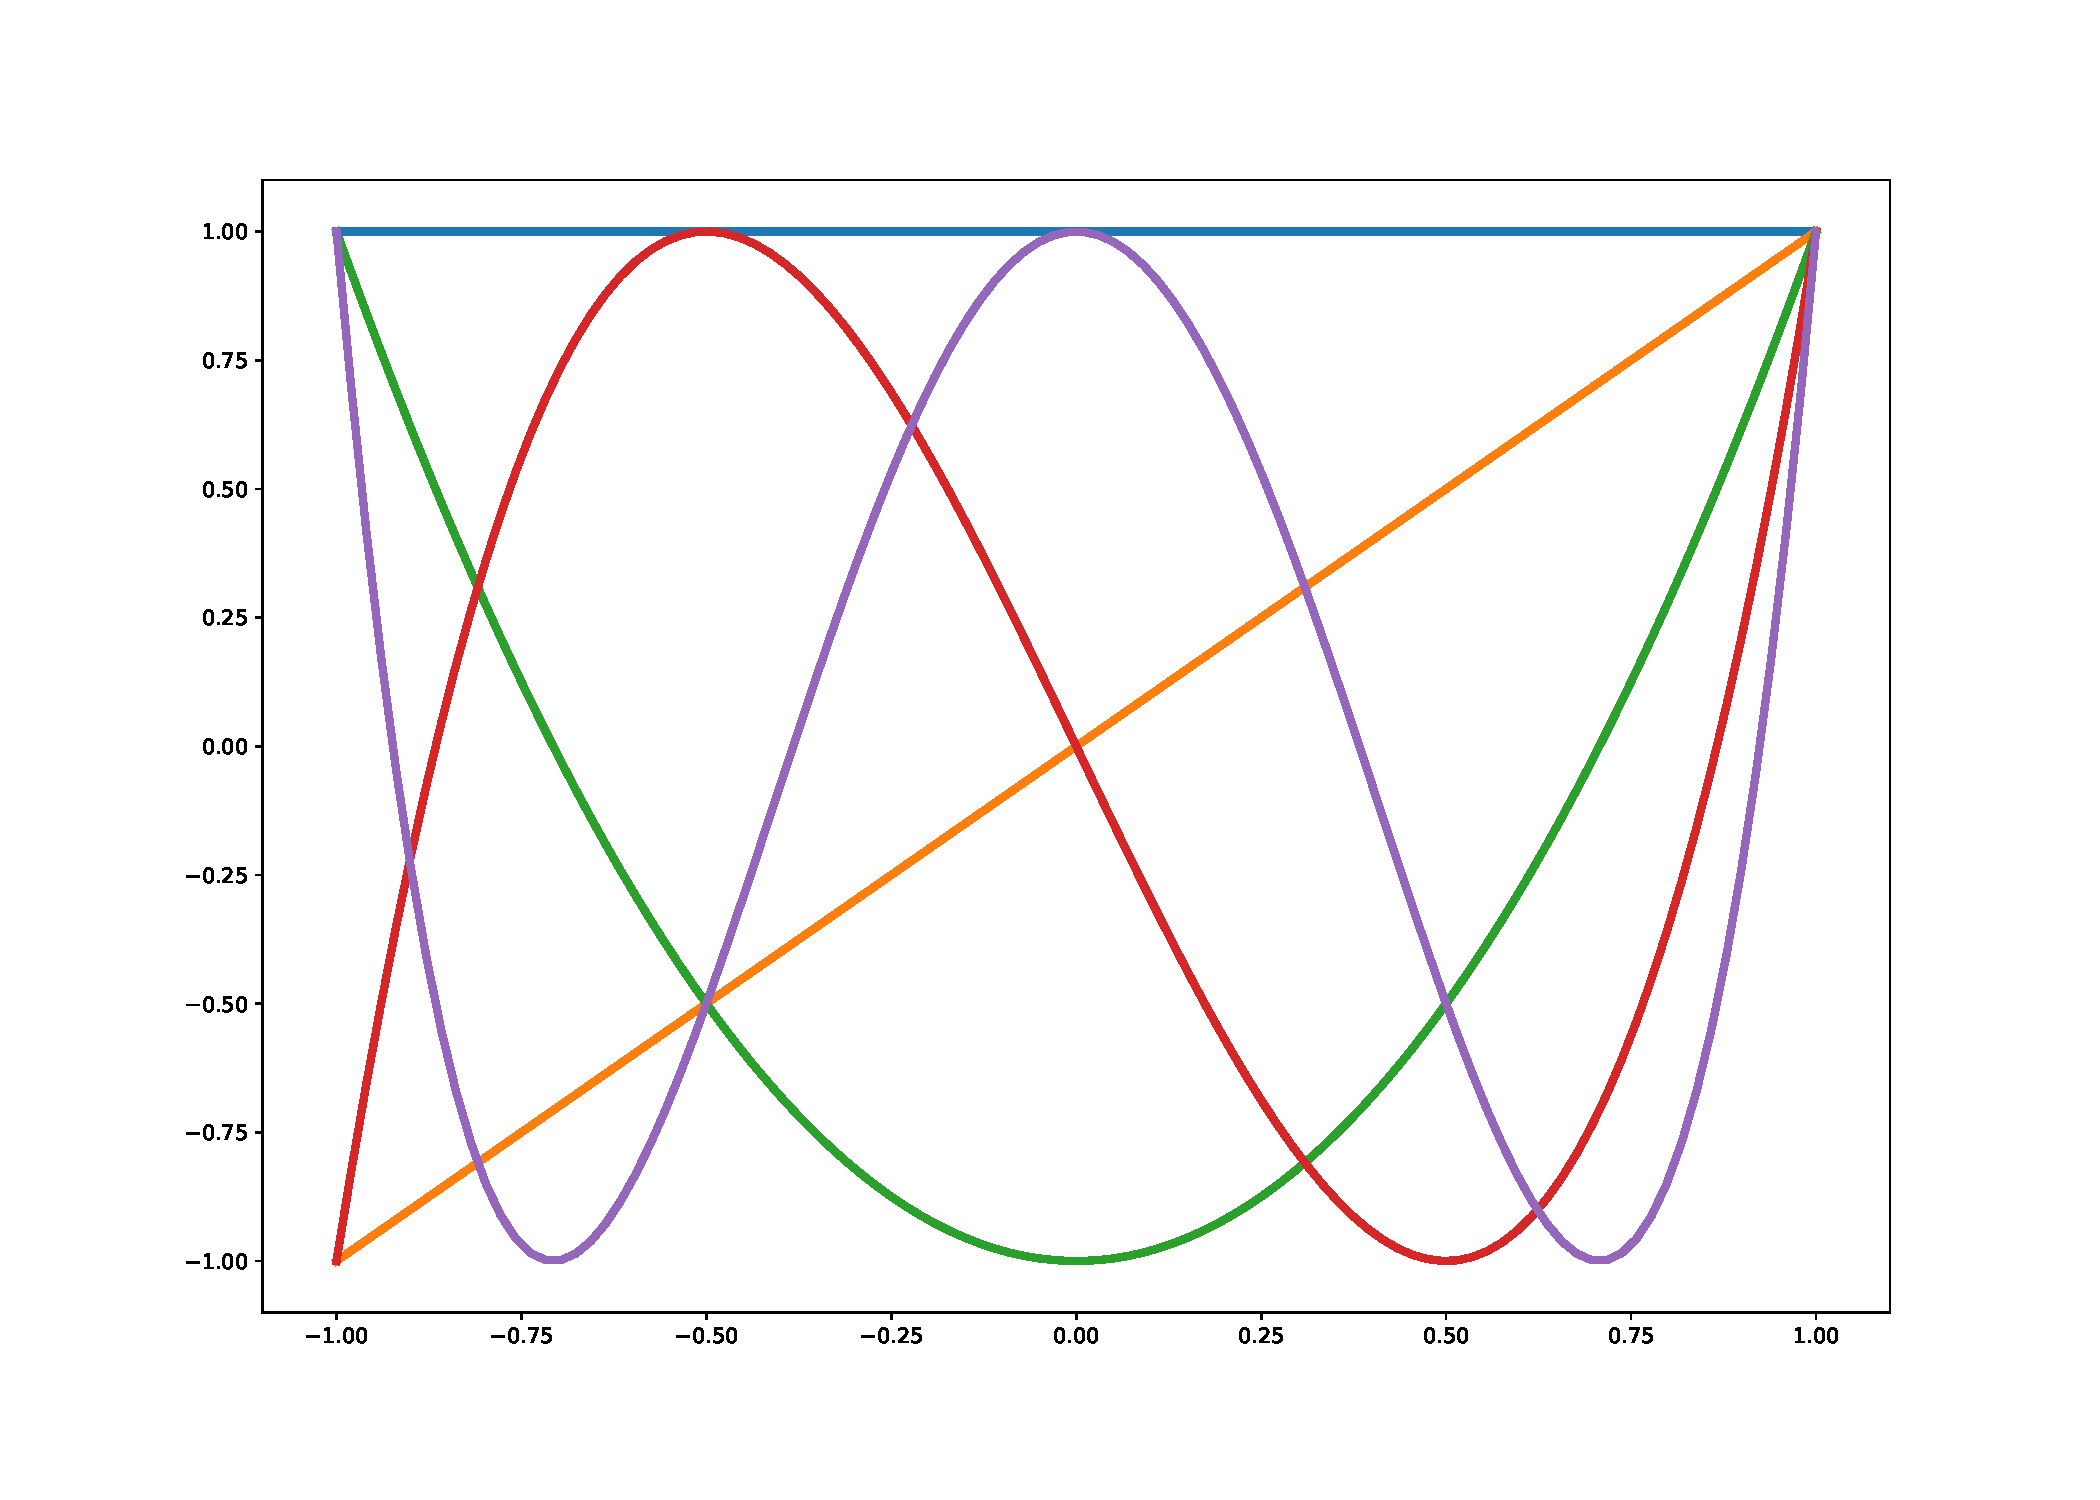
\includegraphics[width=0.9\textwidth]{figures/lecture6-cheb_polynome.pdf}
\centering
\caption{Chebychev polynomials of varying degrees.}
\label{chebychev_poly}
\end{figure}

Why Chebyshev polynomials? Suitably rescaled, they minimize the absolute value in a desired interval $[\alpha, \beta]$ while satisfying the normalization constraint of having value $1$ at the origin.

Recall that the eigenvalues of the matrix we consider are in the interval $[\alpha, \beta]$. We need to rescale the Chebyshev polynomials so that they're supported on this interval and still attain value $1$ at the origin. This is accomplished by the polynomial

\begin{equation*}
P_k(a) = \frac{T_k\left(\frac{\alpha + \beta - 2a}{\beta - \alpha}\right)}{T_k\left(\frac{\alpha + \beta}{\beta - \alpha}\right)}.
\end{equation*}
\begin{figure}[ht]
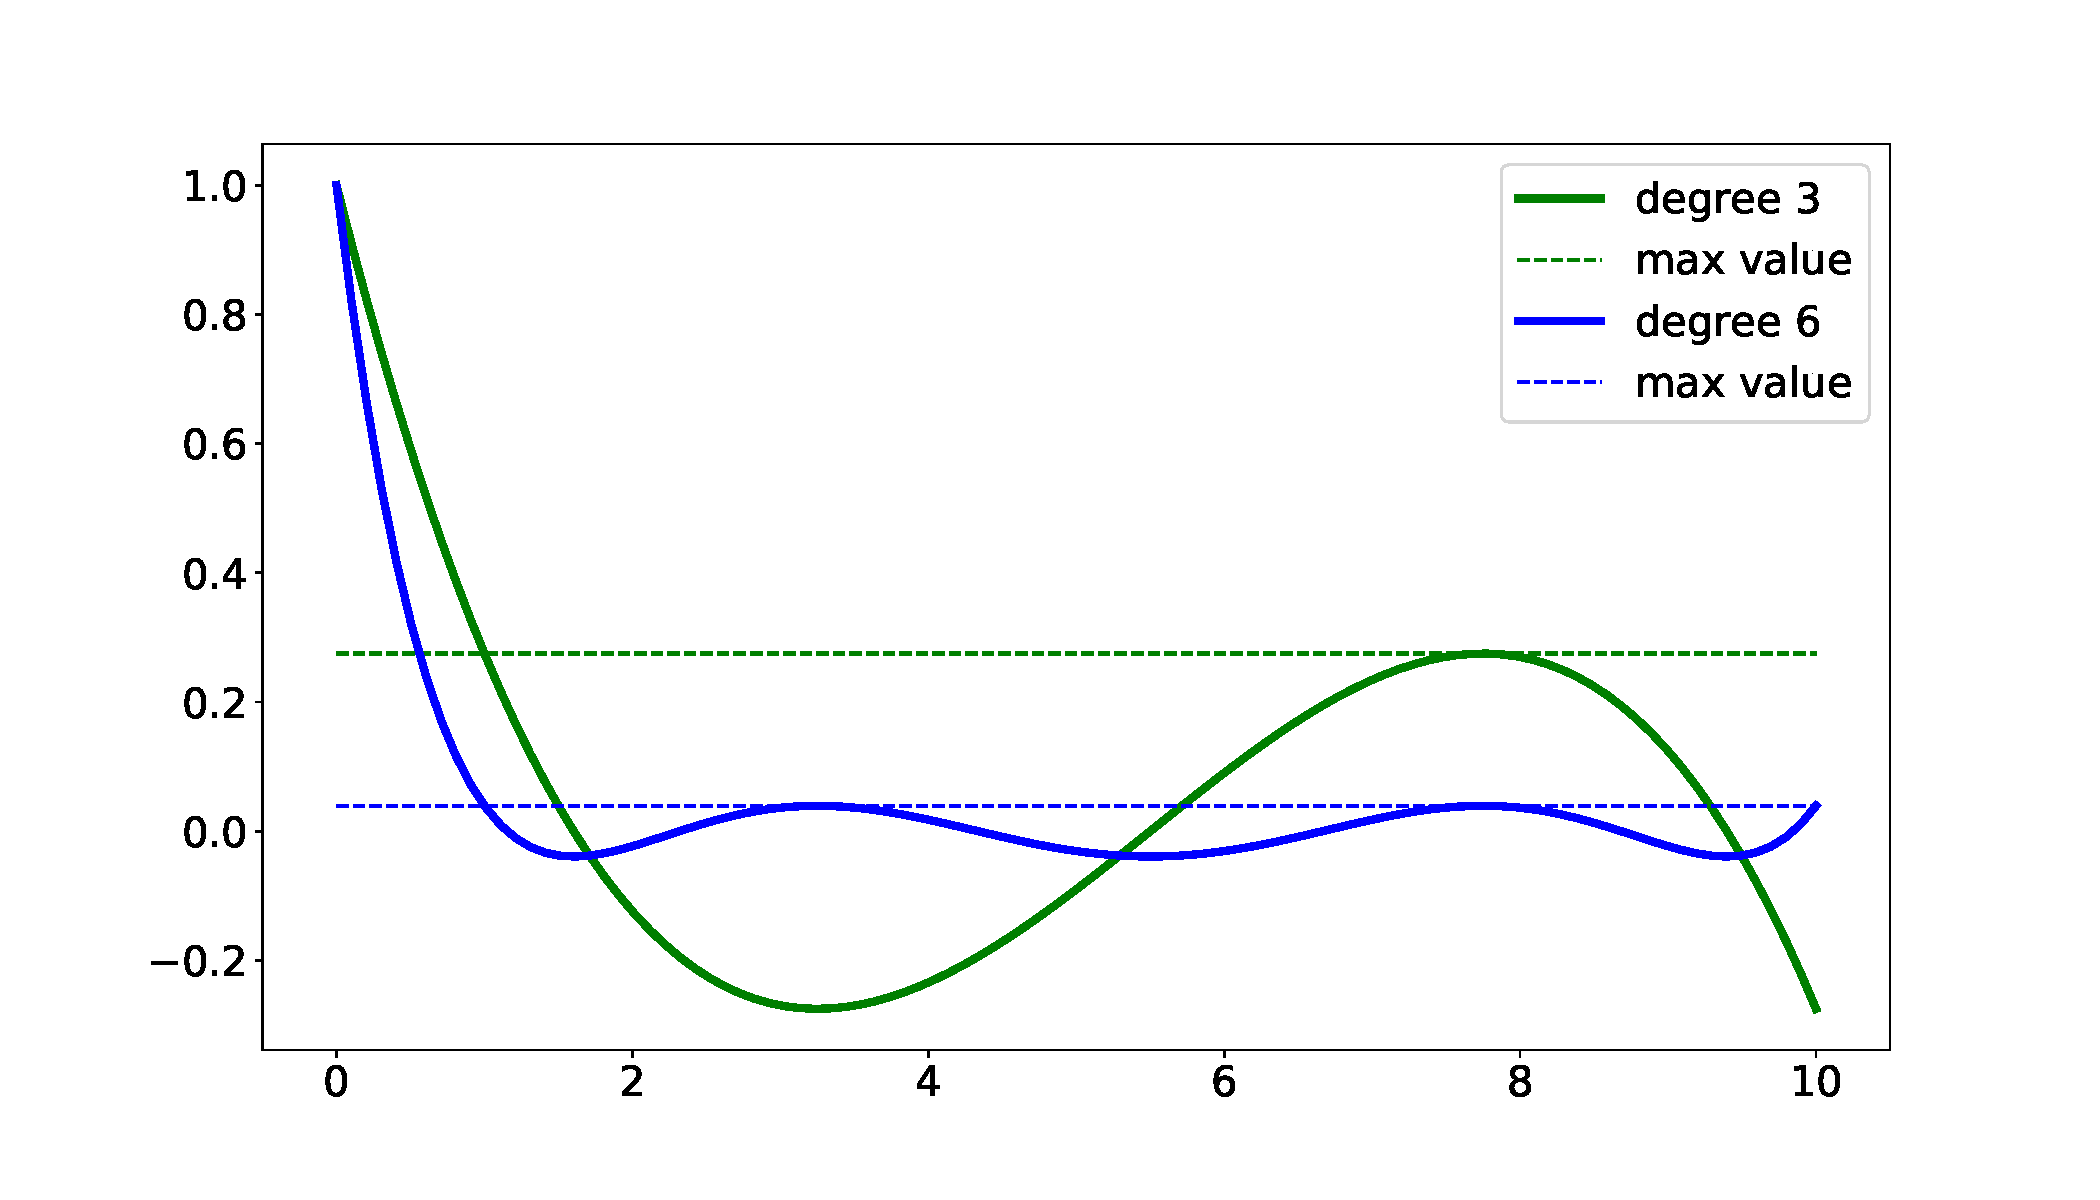
\includegraphics[width=0.9\textwidth]{figures/lecture6-rescaled_cheb.pdf}
\centering
\caption{Rescaled Chebyshev}
\label{rescales_chebyshev}
\end{figure}

\begin{figure}[ht]
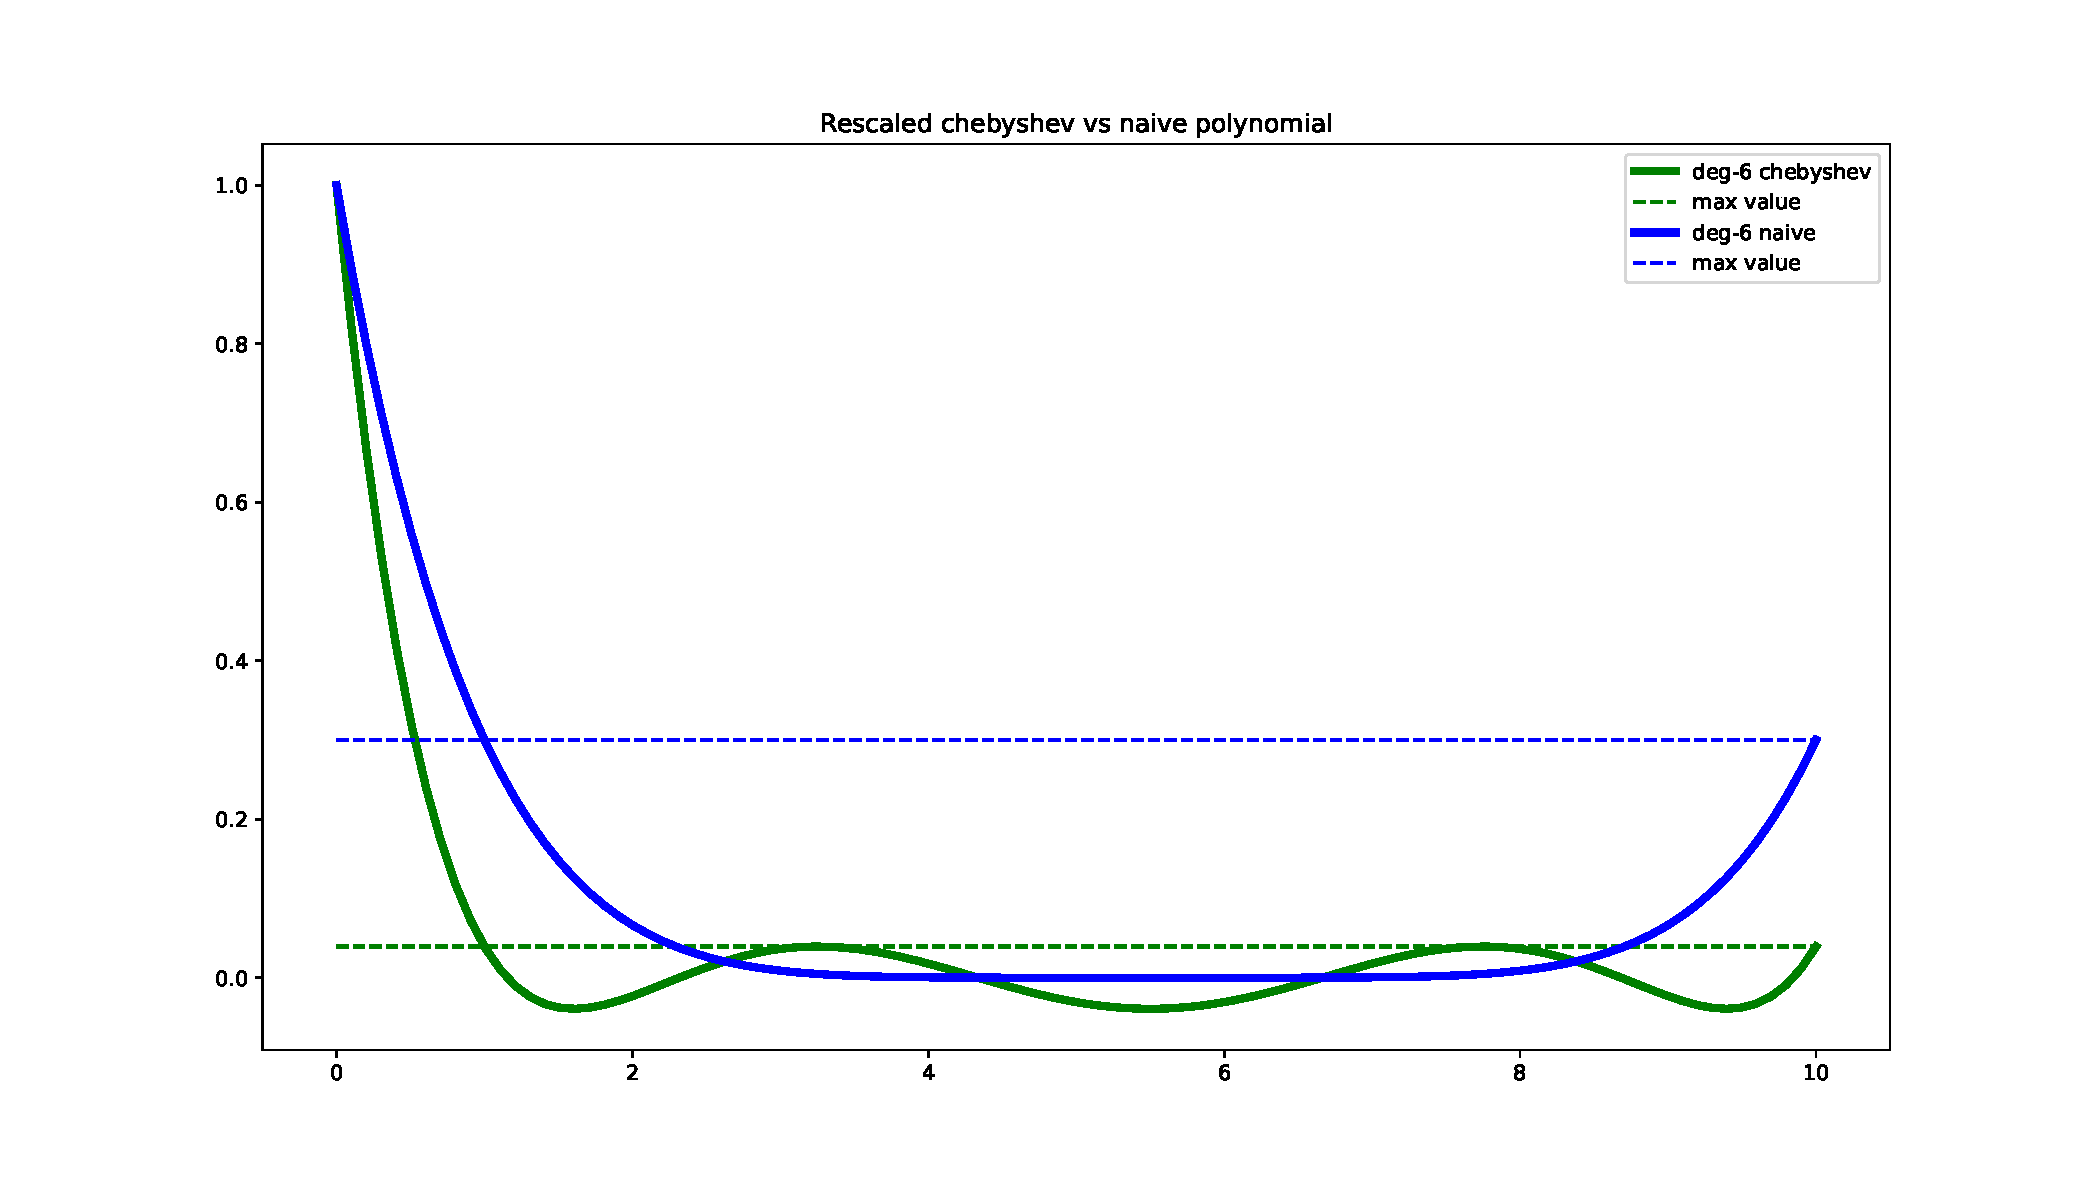
\includegraphics[width=0.9\textwidth]{figures/lecture6-rescaled_cheb_vs_naive.pdf}
\centering
\caption{Rescaled Chebyshev VS Naive Polynomial}
\label{rescaled_chebyshev_vs_naive_p}
\end{figure}

We see on figure \ref{rescales_chebyshev} that doubling the degree has a much more dramatic effect on the magnitude of the polynomial in the interval $[\alpha, \beta].$

Let's compare on figure \ref{rescaled_chebyshev_vs_naive_p} this beautiful Chebyshev polynomial side by side with the naive polynomial we saw earlier. The Chebyshev polynomial does much better: at around 0.3 for degree 3 (needed degree 6 with naive polynomial), and below 0.1 for degree 6.



\subsubsection{Accelerated gradient descent}

The Chebyshev polynomial leads to an accelerated version of gradient descent. Before we describe the iterative process, let's first see what error bound comes out of the Chebyshev polynomial.

So, just how large is the polynomial in the interval $[\alpha, \beta]$? First,
note that the maximum value is attained at $\alpha$. Plugging this into the
definition of the rescaled Chebyshev polynomial, we get the upper bound for any
$a\in[\alpha, \beta],$

\begin{align*}
|P_k(a)| &\leq |P_k(\alpha)| 
= \frac{|T_k(1)|}{|T_K\left(\frac{\beta + \alpha}{\beta - \alpha}\right)|} 
\le \left|T_K\left(\frac{\beta + \alpha}{\beta - \alpha}\right)^{-1}\right|.
\end{align*}
Recalling the condition number $\kappa=\beta/\alpha,$ we have
\begin{equation*}
\frac{\beta + \alpha}{\beta - \alpha} = \frac{\kappa + 1}{\kappa - 1}.
\end{equation*}
Typically $\kappa$ is large, so this is $1 + \epsilon$, $\epsilon \approx \frac{2}{\kappa}$. Therefore, we have
\begin{eqnarray*}
|P_k(a)| &\leq {|T_k(1 + \epsilon)^{-1}|}.
\end{eqnarray*}

To upper bound $|P_k|$, we need to lower bound $|T_k(1 + \epsilon)|$.

\textbf{Fact}: for $a > 1$, $T_k(a) = \cosh\left(k \cdot \mathrm{arccosh} (a)\right)$ where:
\begin{equation*}
\cosh(a) = \frac{e^a + e^{-a}}{2},\quad \mathrm{arccosh}(a) = \ln\left(x + \sqrt{x^2 - 1}\right).
\end{equation*}

Now, letting $\phi = \mathrm{arccosh}(1 + \epsilon)$:
\begin{equation*}
e^{\phi} = 1 + \epsilon + \sqrt{2\epsilon + \epsilon^2} \geq 1 + \sqrt{\epsilon}.
\end{equation*}
So, we can lower bound $|T_k(1 + \epsilon)|$:
\begin{align*}
|T_k(1 + \epsilon)| &= \cosh\left(k \mathrm{arccosh}(1 + \epsilon)\right) \\
&= \cosh(k\phi) \\
&= \frac{(e^\phi)^k + (e^{-\phi})^k}{2} \\
&\geq \frac{(1 + \sqrt{\epsilon})^k}{2}.
\end{align*}

Then, the reciprocal is what we needed to upper bound the error of our algorithm, so we have:
\begin{equation*}
|P_k(a)| \leq {|T_k(1 + \epsilon)^{-1}|} \leq 2(1 + \sqrt{\epsilon})^{-k}.
\end{equation*}

Thus, this establishes that the Chebyshev polynomial achieves the error bound:
\begin{align*}
\left\Vert x_{t+1} - x^* \right\Vert &\leq 2(1 + \sqrt{\epsilon})^{-t}
\left\Vert x_0 -x^*\right\Vert \\
&\approx 2\left(1 + \sqrt{\frac{2}{\kappa}}\right)^{-t} \left\Vert x_0 -x^*\right\Vert \\
&\leq 2\exp\left(-t \sqrt{\frac{2}{\kappa}}\right) \left\Vert x_0 -x^*\right\Vert.
\end{align*}

This means that for large $\kappa,$ we get quadratic savings in the degree we need before the error drops off exponentially. Figure \ref{convergence} shows the different rates of convergence, we clearly see that the 

\begin{figure}[ht]
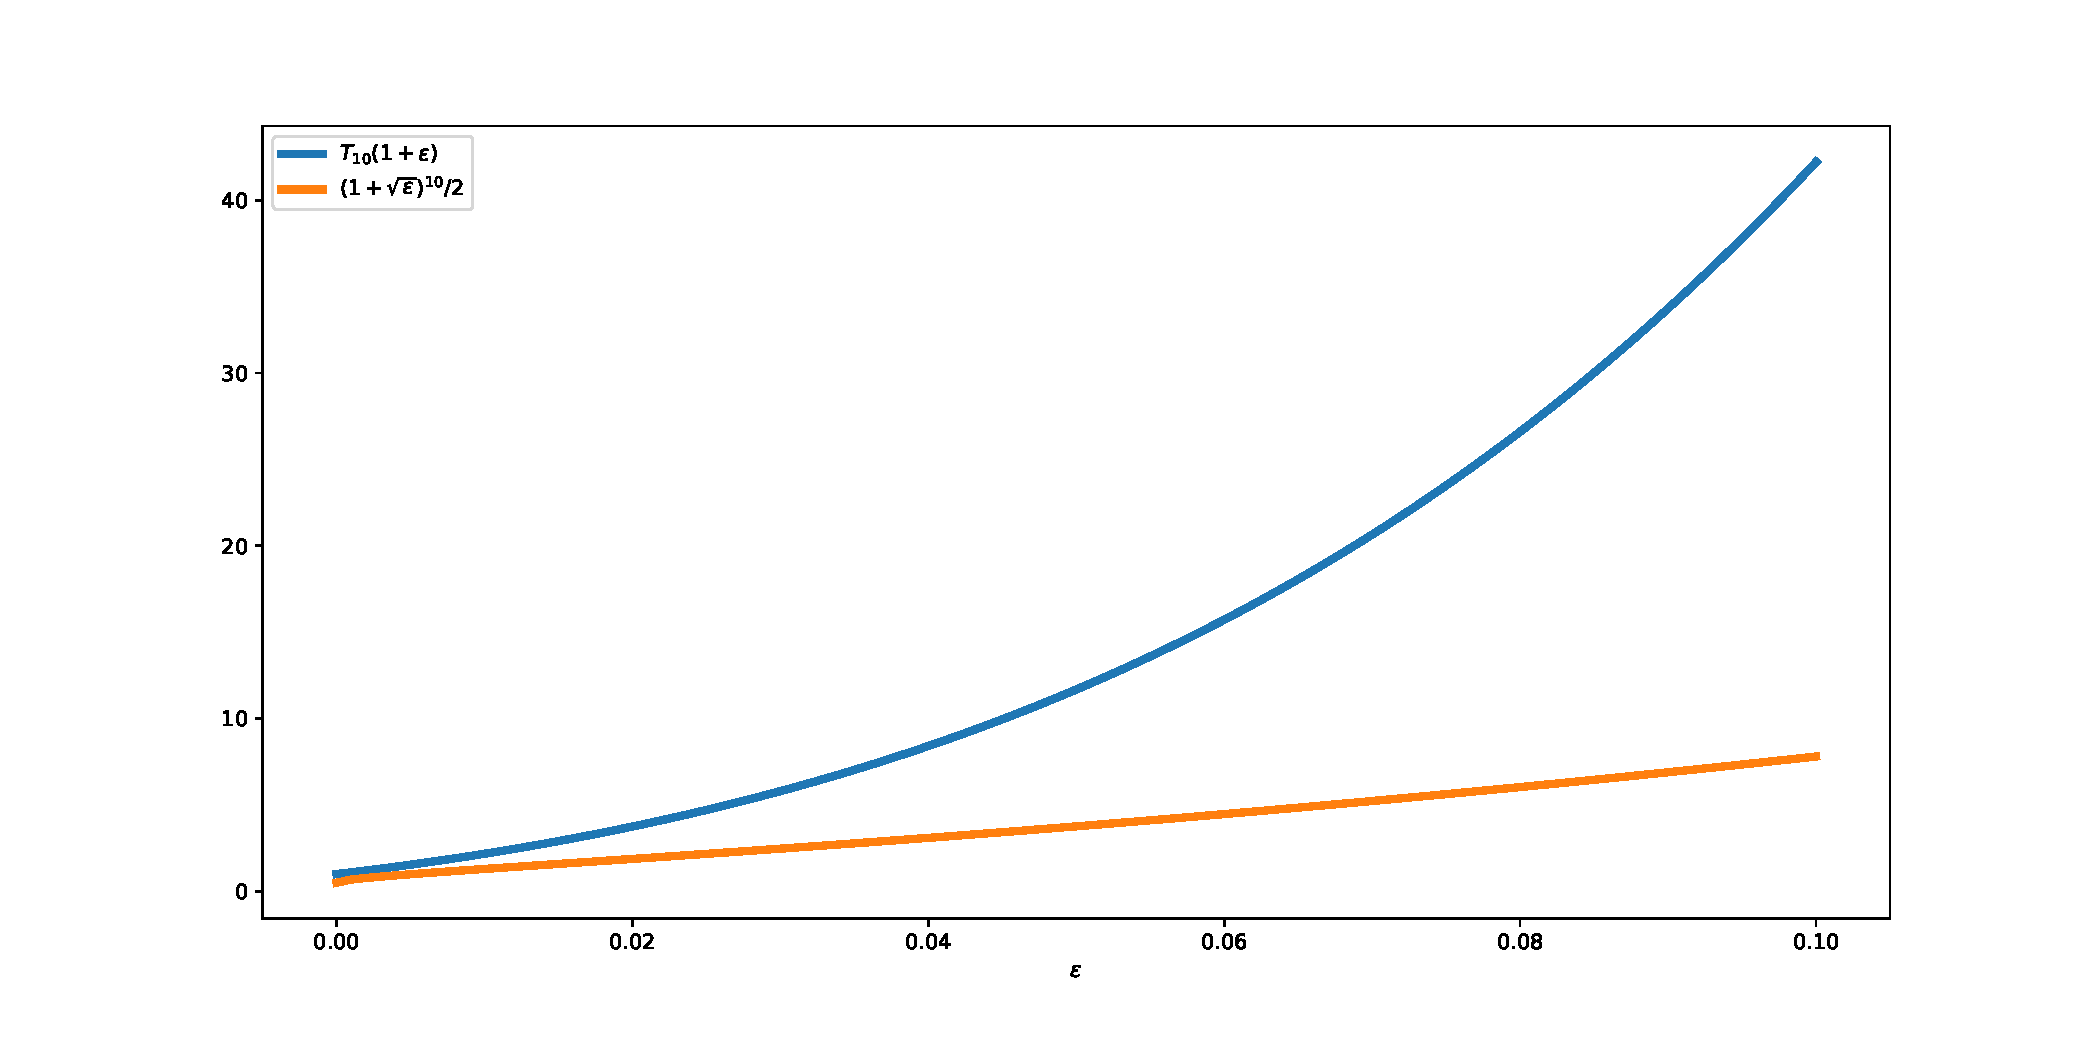
\includegraphics[width=0.9\textwidth]{figures/lecture6-conv.pdf}
\centering
\caption{Convergence for naive polynomial and Chebyshev}
\label{convergence}
\end{figure}

\subsubsection{The Chebyshev recurrence relation}
Due to the recursive definition of the Chebyshev polynomial, we directly get an iterative algorithm out of it. Transferring the recursive definition to our rescaled Chebyshev polynomial, we have:
\begin{equation*}
P_{K+1}(a) = (\eta_k a + \gamma_k)P_k(a) + \mu_k P_{k-1}(a).
\end{equation*}

where we can work out the coefficients $\eta_k,\gamma_k,\mu_k$ from the recurrence definition. Since $P_k(0)=1,$ we must have $\gamma_k+\mu_k=1.$ This leads to a simple update rule for our iterates:

\begin{eqnarray*}
x_{k+1} &= (\eta_k A + \gamma_k)x_k + (1 - \gamma_K)x_{k-1} - \eta_k b \\
&= (\eta_k A + (1 - \mu_k))x_k + \mu_k x_{k-1} - \eta_k b \\
&= x_k - \eta_k(Ax_k - b) + \mu_k(x_k - x_{k-1}).
\end{eqnarray*}

We see that the update rule above is actually very similar to plain gradient descent except for the additional term  $\mu_k(x_k - x_{k-1}).$ This term can be interpreted as a \textit{momentum} term, pushing the algorithm in the direction of where it was headed before. In the next lecture, we'll dig deeper into momentum and see how to generalize the result for quadratics to general convex functions.

